\documentclass[a4paper,12pt,final] {article}
\usepackage{graphicx}
\usepackage{listings}
\usepackage[frenchb]{babel}
\usepackage[T1]{fontenc}
\usepackage[utf8]{inputenc}
\usepackage[autolanguage]{numprint}
\usepackage{eurosym}
\usepackage{makeidx}
\usepackage[pdftex]{hyperref}
\makeindex
\usepackage{float}
\usepackage{tikz}
\usetikzlibrary{shapes}
\usepackage{color}
\usepackage{url}
\usepackage{fancyhdr}
\usepackage{lastpage}
\usepackage{geometry}
\usepackage{url}
\usepackage{pst-node, pstricks}

% for the pictures
\graphicspath{{./include/}} % déclaration du dossier d'enregistrement des photos
\DeclareGraphicsExtensions{.png,.eps,.jpg} % png, jpg etc. ne compile pas en DVI ... préférer l'eps
% enlever les extensions aux photos ?

% for the code
\usepackage{listings}
\definecolor{vert}{rgb}{0.2,0.6,0.4} 
\definecolor{grey}{rgb}{0.95,0.95,0.95}
\lstset{language=c,frame=single, breaklines=true, basicstyle=\ttfamily,backgroundcolor=\color{grey},basicstyle=\scriptsize, keywordstyle=\color{blue}, commentstyle=\color{vert}, stringstyle=\color{red}, identifierstyle=\ttfamily,showstringspaces=false}

\def\subsubsubsection{\paragraph}
\def\subsubsubsubsection{\subparagraph}

\hypersetup{pdfpagemode=none,
pdfstartview=FitH,
pdfkeywords={LaTeX: document typesetting system},
breaklinks=true,
colorlinks=true,
linkcolor=black,
citecolor=black,
filecolor=black,
urlcolor=blue
}


\author{Ludovic Delaveau, Benjamin Loulier}
\title{Plus court chemin dans un graphe}

\lfoot{École Nationale Supérieure des Mines de Saint-Étienne}
\cfoot{}
\rfoot{\thepage/\pageref{LastPage}}
\lhead{Plus court chemin dans un graphe}
\chead{}
\rhead{Loulier - Delaveau}

\pagestyle{fancy}


\geometry{top=2cm}	
\geometry{bottom=3cm} % bottom margin

\begin{document}

% page de garde
\begin{titlepage}

\vspace*{\fill} % pour remplir le haut de la page
    \hspace*{\fill}

\begin{center}

\centering
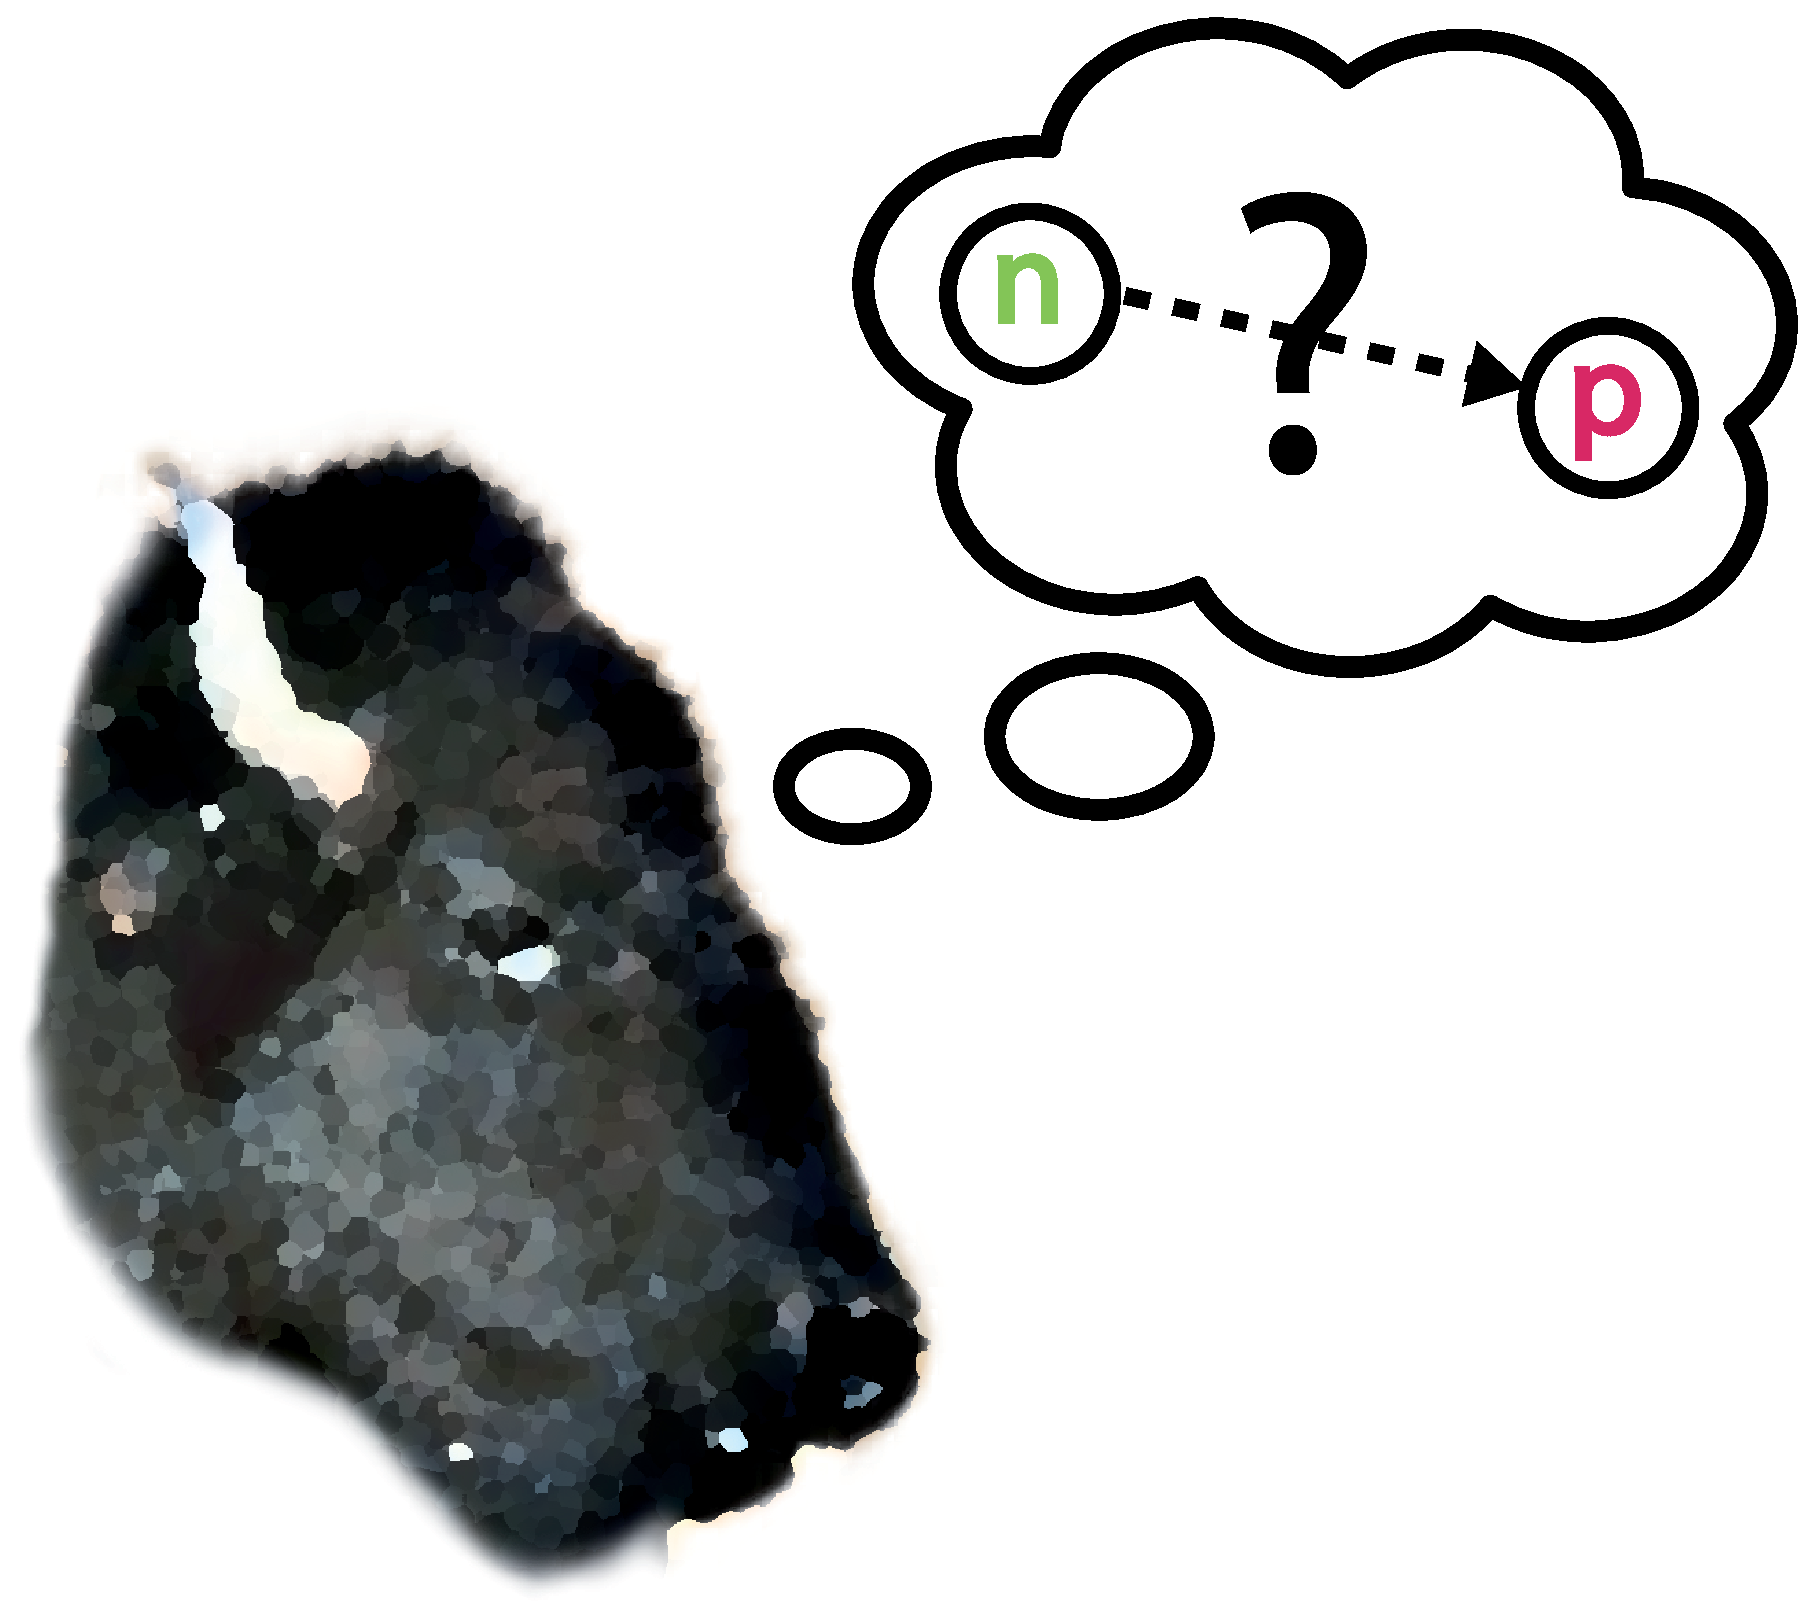
\includegraphics[scale=0.3]{icone}\\[2cm] % bison fûté

% Title
\rule{15cm}{0.2mm} \\[0.4cm]
{ \huge \bfseries Plus court chemin dans un graphe}\\[0.4cm]
 \rule{15cm}{0.2mm} \\[0.4cm]

\begin{minipage}{0.4\textwidth}
\begin{flushleft} \large
\emph{Auteurs :}\\
Benjamin \textsc{Loulier}\\
Ludovic \textsc{Delaveau}\\
\end{flushleft}
\end{minipage}
\begin{minipage}{0.4\textwidth}
\begin{flushright} \large
\emph{Tuteurs :} \\
Roland \textsc{Jegou}\\
Michel \textsc{Beigbeder}\\
\end{flushright}
\end{minipage}
 
\vfill
Projet d'Axe informatique 2009-2010
\end{center}

\end{titlepage}

\newpage

\setcounter{page}{2} 
\tableofcontents

\newpage

\section{Introduction}

Le fait de trouver le plus court chemin dans un graphe (pathfinding en anglais) trouve énormément d'applications dans l'industrie. Un premier exemple d'application qui nous vient à l'esprit est évidemment les utilisations faites dans les GPS pour le calcul d'itinéraires, avec une valuation donnée en fonction de la distance d'un axe, mais également en fonction de l'importance de l'axe, voire même en fonction du trafic et de l'encombrement. D'autres utilisations moins connues sont par exemple les algorithmes associés au routage des données dans un réseau (application très sensible et nécessitant des algorithmes les plus performants possible, afin d'optimiser les temps de réponse entre les routeurs) ou à de l'optimisation de process.\\

Le travail fait ici s'appuie sur les graphes orientés valués, qui sont une forme de graphe la plus générique, et les algorithmes implémentés peuvent très facilement s'adaptés à des graphes non-orientés.\\

Nous avons pris le parti dans ce projet de ne traiter que des algorithmes trouvant exactement le chemin le plus court et pas un chemin optimisé. Nous avons décidé de ne pas utiliser des algorithmes approchés tels que A* car nous les avons déjà traité en première année dans le cadre du cours de java. Nous avons donc étudié trois algorithmes : L'algorithme de Bellman-Ford, l'algorithme de Dijkstra et l'algorithme de Dantzig.\\

Ce rapport se divise en trois parties principales, présentant d'abord les graphes ainsi que les structures de données que nous avons utilisées, puis les algorithmes que nous avons implémentés. Enfin l'application que nous avons réalisée sera présentée.

\newpage
\section{Définitions et structures de données}
\subsection{Graphe}

Un graphe simple est un couple formé de deux ensembles: \\
$$G=(X,A)$$ avec X l'ensemble des sommets, et A l'ensemble des arêtes.\\
$$G=(X,A,v)$$ si on ajoute la possibilité de donner une valeur différentes aux arêtes, nous avons dans ce cas un graphe valué et v est l'ensemble des valuations.\\
Un graphe peut être non orienté, auquel cas une arête entre un sommet A et B permet aussi bien de se rendre de A en B et de en A. Il peut être aussi orienté, dans ce cas une arête ne peut être parcourue que dans un sens.

\begin{figure}[htdp]
\begin{psmatrix}[mnode=circle]
         &   &   & C & E            \\
$\alpha$ & A & B & D &   & $\omega$ \\
         &   &   & F
\end{psmatrix}

\psset{arrows=->,
       labelsep=1mm,
       shortput=nab}

\ncline{2,1}{2,2}^{0} 
\ncline{2,2}{2,3}^{2} 
\ncline{2,3}{1,4}^{4} 
\ncline{2,3}{2,4}^{4} 
\ncline{2,3}{3,4}^{4}
\ncline{1,4}{1,5}^{3}
\ncarc[arcangle=10]{2,4}{1,5}^{2}
\ncarc[arcangle=10]{1,5}{2,4}^{2}
\ncline{3,4}{2,6}^{4}
\ncline{1,5}{2,6}^{10}

\caption{Exemple de graphe valué orienté}
\end{figure}
\subsection{Matrice d'adjacence}

plop
\begin{figure}[htdp]
\begin{center}
\begin{tabular}{|c|c|c|}
\hline
0 & 4 & $\infty$\\
\hline
8 & 0 & 3 \\
\hline
42 & $\infty$ & 0 \\
\hline
\end{tabular}
\end{center}
\caption{matrice d'adjacence}
\end{figure}%

Dans notre programme nous avons utilisé un tableau d'entiers, qui sont alloués dynamiquement puisque la taille du graphe est déterminée pendant l'exécution par l'utilisateur :
\begin{lstlisting}
int ** matrix;
\end{lstlisting}

\subsection{Tableau de liste chaînées}

Voilà la définition utilisée dans notre programme de la structure de données de liste chaînées :
\begin{lstlisting}
struct chained_list {
	int number;
	int value;
	struct chained_list * next;
};
\end{lstlisting}

Nous utilisons un tableau de liste chaînées, dont la déclaration est :
\begin{lstlisting}
struct chained_list ** list;
\end{lstlisting}
Il s'agit d'un double pointeur, puisqu'il est alloué également dynamiquement, pour les mêmes raisons que la matrice d'adjacence.

\subsection{Matrice de prédécesseur}

La matrice de prédécesseurs est l'une des deux structures de données utilisées en tant que structure de données de sortie. Elle est utilisée dans les algorithmes de Bellman-Ford et de Dijkstra, ainsi que dans une certaine mesure dans celui de Dantzig, comme nous le verrons par la suite.\\

Une matrice de prédécesseur est définie pour un noeud de départ donné. Cette matrice, telle que nous l'avons implémentée dans notre programme est de dimension ``nombre de noeuds" * 2, et stocke pour un noeud de départ donné ses prédécesseurs et les distances associées. La première colonne contient les poids des arcs qui relient le noeud de départ à la deuxième colonne, qui contient les prédécesseurs. On donne un poids nul à l'arc reliant le noeud de départ  à lui-même, et on indique $\infty$ comme prédecesseur.\\

La figure 3 donne la matrice de prédécesseur du noeud 0 du graphe décrit par la matrice d'adjacence donnée en exemple à la figure 2.\\ % attention au numéro !

\begin{figure}[htdp]
\begin{center}
\begin{tabular}{|c|c|}
\hline
0 &$\infty$\\
\hline
4 & 1 \\
\hline
$\infty$ & $\infty$ \\
\hline
\end{tabular}
\end{center}
\caption{Matrice de prédécesseur pour le noeud 0 de la figure 2}
\end{figure}%

Le code utilisé pour définir la matrice n'est pas différent de celui de la matrice d'adjacence. La taille est toujours donnée dynamiquement, avec la différence cette fois que la matrice n'a que deux colonnes.
\begin{lstlisting}
int ** predecessor_matrix;
\end{lstlisting}

\subsection{``Matrice de Dantzig"}

Cette matrice, qui est comme son nom l'indique utilisée dans l'algorithme de Dantzig pour collecter les résultats, est une matrice ``nombre de noeuds" * ``nombre de noeuds" * 2. Dantzig, comme nous le verrons par la suite travaille sur le graphe entier, faisant  le calcul sur tous les sommets.\\

Dès lors, tel que nous avons implémenté la matrice, il s'agit simplement d'un tableau de n matrices de prédécesseurs, où n est le nombre de noeuds dans le graphe.\\

La figure 4 présente un exemple de cette matrice pour la matrice d'adjacence donnée à la figure 2. La matrice n'est ici pas le résultat d'un calcul de l'algorithme, et des chemins possibles n'y figurent pas, tandis que des chemins plus courts ne sont pas notés.\\ % attention au numéro !

\begin{figure}[htdp]
\begin{center}
\begin{tabular}{|c|c|c|}
\hline
(0, $\infty$) & (4, 1) & ($\infty$, $\infty$) \\
\hline
(8, 0) & (0, $\infty$) & (3, 2)\\
\hline
(42, 0) & ($\infty$, $\infty$) & (0, $\infty$)\\ 
\hline
\end{tabular}
\end{center}
\caption{Matrice utilisée dans l'algorithme de Dantzig}
\end{figure}

L'implémentation d'une telle matrice est faite également très simplement, suivant ce qui est fait pour la matrice de prédécesseur. On a ici une matrice à trois dimensions, et donc un triple pointeur sur un entier :
\begin{lstlisting}
int *** matrix;
\end{lstlisting}

\subsection{choix des types de données}

Nous avons choisi d'utiliser des entiers pour représenter à la fois les noeuds et aussi leur valeur. Il nous a en effet semblé suffisant de se limiter à INT\_MAX en terme de nombre de noeuds. Cela représente tout de même \nombre{2147483647} noeuds, et une plage de valuation suffisante. La machine sera tout de façon d'abord limitée en terme d'espace mémoire pour les représenter.\\

Dans l'implémentation des algorithmes nous avons surtout utilisé des matrices, par la rapidité de temps d'accès qu'elles permettent, et aussi par la simplicité de l'implémentation qu'elles permettent. Gérer une liste sans index est en effet plus compliqué, avec des algorithmes qui utilisent en permanence des valeurs stockées précédemment. Nous le verrons par la suite, mais tous les algorithmes se servent des valeurs déjà calculées, ou remplacent celles déjà stockées.\\

\newpage
\section{Présentation des trois algorithmes}

Nous avons donc implémenté les trois algorithmes principaux de recherche de chemins, qui sont ceux de Bellman-Ford, de Dijkstra et de Dantzig. Chacun a ses propres particularités, en particulier en terme de champ d'application.\\

Dans la suite de cette partie, nous allons étudier les différents algorithmes sur un même exemple, dont la matrice d'adjacence et la représentation sont données aux figures 5 et 6.\\ % attention au numéro !

\begin{figure}[htpd]
 \centering
 \begin{psmatrix}[mnode=circle]
	    & 2\\
	 1 &    & 4\\
	    & 3\\
\end{psmatrix}
	
\psset{arrows=->, labelsep=1mm, shortput=nab}
	\ncline{2,1}{1,2}^{6}
	\ncline{2,1}{3,2}^{1}
	\ncline{1,2}{2,3}^{1}
	\ncline{3,2}{1,2}^{1}
	\ncline{3,2}{2,3}^{1}

  \caption{Le graphe qui est utilisé dans les sections suivantes}
\end{figure}

\begin{figure}[htpd]
\begin{center}
\begin{tabular}{|c|c|c|c|}
\hline
0 & 6 & 1 & $\infty$\\
\hline
$\infty$ & 0 & $\infty$ & 1\\
\hline
$\infty$ & 1 & 0 & 1\\
\hline
$\infty$ & $\infty$ & $\infty$ & 0\\
\hline
\end{tabular}
\end{center}
\caption{La matrice d'adjacence associée au graphe de la figure précédente}
\end{figure}

%%%%%%%%%%%%Fin de l'intro de la partie 3%%%%%%%%%%%
\subsection{Bellman-Ford}
Bellman-Ford permet de trouver la matrice de prédécesseur pour un point de départ donné et permet de trouver un plus court chemin dans un graphe circuit contenant des valuations positives et/ou negatives.\\
Bellman Ford fonctionne en regardant pour chaque sommet du graphe les prédécesseurs et en comparant les poids affectés à chaque sommet. Voici le pseudo code de l'algorithme de Bellman-Ford.
\begin{lstlisting}
 bool Bellman_Ford( G, s) 
 
   initialisation ( G, s)  // les poids de tous les sommets sont mis a +infini 
                           // le poids du sommet initial a 0
   compteur = 0
   tant que des modifications sont faites
   	pour i=1 a Nombre de sommets -1 faire
        		pour chaque predecesseur j de i faire
           		paux := poids(j) + poids(arc(i, j)); 
           		si paux < poids(i) alors
               			pred(i) := j; 
               			poids(i) := paux; 
         si compteur > Nombre de sommets et si il y a eu des modifications
   		retourner `Le graphe contient des circuits`
\end{lstlisting}

Voici le déroulement de l'algorithme de Bellman-Ford sur un graphe d'exemple.

\begin{figure}[htpd]
\begin{center}
\begin{psmatrix}[mnode=circle]
 & 2\\
 1\\
 & 3\\
\end{psmatrix}

\psset{arrows=->, labelsep=1mm, shortput=nab}
	\ncline{2,1}{1,2}^{6}
	\ncline{2,1}{3,2}^{1}
	\ncline{3,2}{1,2}^{3}

\end{center}
\caption{Etat initial}
\end{figure}

\begin{figure}[htpd]
\begin{center}
\begin{tabular}{|c|c|c|c|}
\hline
1 & 0 & - \\
\hline
2 & $\infty$ & - \\
\hline
3 & $\infty$ & - \\
\hline
\end{tabular}
\end{center}
\caption{Matrice de predecesseur pour l'etat initial}
\end{figure}
%Etape 1
On va visiter le sommet 2 ensuite et on regarde son premier prédecesseur 1.
\begin{figure}[htpd]
\begin{center}
\begin{psmatrix}[mnode=circle]
 & {\color{red} \bf 2}\\
 1\\
 & 3\\
\end{psmatrix}

\psset{arrows=->, labelsep=1mm, shortput=nab}
	\ncline[linewidth=2pt]{2,1}{1,2}^{6}
	\ncline{2,1}{3,2}^{1}
	\ncline{3,2}{1,2}^{3}

\end{center}
\caption{Etape 1}
\end{figure}

\begin{figure}[htpd]
\begin{center}
\begin{tabular}{|c|c|c|c|}
\hline
1 & 0 & - \\
\hline
{\color{red} \bf 2} & 6 & 1 \\
\hline
3 & $\infty$ & - \\
\hline
\end{tabular}
\end{center}
\caption{Matrice de predecesseur pour l'Etape 1}
\end{figure}
%Etape 2
On regarde le deuxième prédecesseur de 2 qui est 3, rien ne change.
\begin{figure}[htpd]
\begin{center}
\begin{psmatrix}[mnode=circle]
 & {\color{red} \bf 2}\\
 1\\
 & 3\\
\end{psmatrix}

\psset{arrows=->, labelsep=1mm, shortput=nab}
	\ncline{2,1}{1,2}^{6}
	\ncline{2,1}{3,2}^{1}
	\ncline[linewidth=2pt]{3,2}{1,2}^{3}

\end{center}
\caption{Etape 2}
\end{figure}

\begin{figure}[htpd]
\begin{center}
\begin{tabular}{|c|c|c|c|}
\hline
1 & 0 & - \\
\hline
{\color{red} \bf 2} & 6 & 1 \\
\hline
3 & $\infty$ & - \\
\hline
\end{tabular}
\end{center}
\caption{Matrice de predecesseur pour l'Etape 2}
\end{figure}
%Etape 3
On regarde le sommet 3 et son unique prédecesseur 1.
\begin{figure}[htpd]
\begin{center}
\begin{psmatrix}[mnode=circle]
 & 2\\
 1\\
 & {\color{red} \bf 3}\\
\end{psmatrix}

\psset{arrows=->, labelsep=1mm, shortput=nab}
	\ncline{2,1}{1,2}^{6}
	\ncline[linewidth=2pt]{2,1}{3,2}^{1}
	\ncline{3,2}{1,2}^{3}

\end{center}
\caption{Etape 3}
\end{figure}

\begin{figure}[htpd]
\begin{center}
\begin{tabular}{|c|c|c|c|}
\hline
1 & 0 & - \\
\hline
2 & 6 & 1 \\
\hline
{\color{red} \bf 3} & $ 1 $ & 1 \\
\hline
\end{tabular}
\end{center}
\caption{Matrice de predecesseur pour l'Etape 3}
\end{figure}
%Etape 4
Tous les sommets ont été visités et des modifications ont été faites on recommence donc avec le sommet 2. Si l'on regarde le premier prédecesseur 1 la situation ne change pas ce qui n'est pas le cas si l'on regarde le deuxième prédecesseur de 2 c'est à dire 3.
\begin{figure}[htpd]
\begin{center}
\begin{psmatrix}[mnode=circle]
 & {\color{red} \bf 2}\\
 1\\
 & 3\\
\end{psmatrix}

\psset{arrows=->, labelsep=1mm, shortput=nab}
	\ncline[linewidth=2pt]{2,1}{1,2}^{6}
	\ncline{2,1}{3,2}^{1}
	\ncline{3,2}{1,2}^{3}

\end{center}
\caption{Etape 4}
\end{figure}

\begin{figure}[htpd]
\begin{center}
\begin{tabular}{|c|c|c|c|}
\hline
1 & 0 & - \\
\hline
{\color{red} \bf 2} & 4 & 3 \\
\hline
3 & $ 1 $ & 1 \\
\hline
\end{tabular}
\end{center}
\caption{Matrice de prédecesseur pour l'Etape 4}
\end{figure}
Si l'on continue de dérouler l'algorithme plus aucune modification ne sera effectuée, nous avons donc trouvé un plus court chemin.

Pour un graphe sans circuit la boucle tant que ne peut pas être parcourue plus de n fois, cette condition nous permet donc de détecter des circuits.

La complexité de cet algorithme est en $o(n^{3})$ dans le pire des cas (graphe complet et boucle tant que parcourue n fois).
%%%%%%%%%%%%%Fin de bellman%%%%%%%%%%%%%%%
\subsection{Dijkstra}
Dijkstra permet de trouver la matrice de prédécesseur pour un point de départ donné (identique à Bellman-Ford) et permet de trouver un plus court chemin dans un graphe contenant seulement des valuations positives.\\
Cette fois-ci Dijkstra regarde les successeurs de chaque sommet, le postulat de base de Dijkstra est que pour trouver un plus court chemin il faut passer par le sommet le plus proche de celui où l'on se trouve. Ce qui n'est pas toujours le cas pour un graphe contenant des valuations négatives, par exemple :
\begin{figure}[htpd]
\begin{center}
\begin{psmatrix}[mnode=circle]
 & 2\\
 1\\
 & 3\\
\end{psmatrix}
\psset{arrows=->, labelsep=1mm, shortput=nab}
	\ncline{2,1}{1,2}^{6}
	\ncline{2,1}{3,2}^{8}
	\ncline{3,2}{1,2}^{-5}

\end{center}
\caption{Graphe avec des valuations négatives}
\end{figure}

Voici le pseudo-code de l'algorithme de Dijkstra.
\begin{lstlisting}
fonction Dijkstra (noeuds, fils, distance, debut, fin)
     Pour n parcourant noeuds
         n.parcouru = infini   // Peut etre implemente avec -1
         n.precedent = 0
     Fin pour
     debut.parcouru = 0
     PasEncoreVu = noeuds
     Tant que PasEncoreVu != liste vide
         n1 = minimum(PasEncoreVu)   // Le noeud dans PasEncoreVu avec parcouru le plus petit
         PasEncoreVu.enlever(n1)
         Pour n2 parcourant fils(n1)   // Les noeuds relies a n1 par un arc
             Si n2.parcouru > n1.parcouru + distance(n1, n2)   // distance correspond au poids de l'arc reliant n1 et n2
                 n2.parcouru = n1.parcouru + distance(n1, n2)
                 n2.precedent = n1   // Dit que pour aller a n2, il faut passer par n1
             Fin si
         Fin pour
     Fin tant que
     chemin = liste vide
     n = fin
     Tant que n != debut
         chemin.ajouterAvant(n)
         n = n.precedent
     Fin tant que
     chemin.ajouterAvant(debut)
     Retourner chemin
 Fin fonction Dijkstra
\end{lstlisting}

Déroulons l'algorithme de Dijkstra sur un exemple.\\
On visite le sommet 1 :
\begin{itemize}
\item Sommets visités : 1
\item Sommets atteignables : 2,3
\end{itemize}

\begin{figure}[htpd]
 \centering
 \begin{psmatrix}[mnode=circle]
	    & 2\\
	 {\color{red} \bf 1} &    & 4\\
	    & 3\\
\end{psmatrix}
	
\psset{arrows=->, labelsep=1mm, shortput=nab}
	\ncline{2,1}{1,2}^{6}
	\ncline{2,1}{3,2}^{1}
	\ncline{1,2}{2,3}^{1}
	\ncline{3,2}{1,2}^{1}
	\ncline{3,2}{2,3}^{1}

  \caption{Etat initial}
\end{figure}

\begin{figure}[htpd]
\begin{center}
\begin{tabular}{|c|c|c|c|}
\hline
 {\color{red} \bf 1} & 0 & - \\
\hline
2 & $\infty$ & - \\
\hline
3 & $\infty$ & - \\
\hline
4 & $\infty$ & - \\
\hline
\end{tabular}
\end{center}
\caption{Matrice de prédecesseur pour l'Etat initial}
\end{figure}
%Etape1
Le sommet le plus proche est le sommet 3 on va donc le visiter.
\begin{itemize}
\item Sommets visités : 1, 3
\item Sommets atteignables : 2, 4
\end{itemize}
\begin{figure}[htpd]
 \centering
 \begin{psmatrix}[mnode=circle]
	    & 2\\
	1 &    & 4\\
	    &  {\color{red} \bf 3}\\
\end{psmatrix}
	
\psset{arrows=->, labelsep=1mm, shortput=nab}
	\ncline{2,1}{1,2}^{6}
	\ncline{2,1}{3,2}^{1}
	\ncline{1,2}{2,3}^{1}
	\ncline{3,2}{1,2}^{1}
	\ncline{3,2}{2,3}^{1}

  \caption{Etape 1}
\end{figure}

\begin{figure}[htpd]
\begin{center}
\begin{tabular}{|c|c|c|c|}
\hline
 1 & 0 & - \\
\hline
2 & 6 & 1 \\
\hline
{\color{red} \bf 3} & 1 & 1 \\
\hline
4 & $\infty$ & - \\
\hline
\end{tabular}
\end{center}
\caption{Matrice de prédecesseur pour l'Etape 1}
\end{figure}
%Etape 2
Le sommet le plus proche non visité est alors 2, on le visite.
\begin{itemize}
\item Sommets visités : 1, 3, 2
\item Sommets atteignables : 4
\end{itemize}
\begin{figure}[htpd]
 \centering
 \begin{psmatrix}[mnode=circle]
	    & {\color{red} \bf 2}\\
	1 &    & 4\\
	    &  3\\
\end{psmatrix}
	
\psset{arrows=->, labelsep=1mm, shortput=nab}
	\ncline{2,1}{1,2}^{6}
	\ncline{2,1}{3,2}^{1}
	\ncline{1,2}{2,3}^{1}
	\ncline{3,2}{1,2}^{1}
	\ncline{3,2}{2,3}^{1}

  \caption{Etape 2}
\end{figure}

\begin{figure}[htpd]
\begin{center}
\begin{tabular}{|c|c|c|c|}
\hline
 1 & 0 & - \\
\hline
{\color{red} \bf 2} & 2 & 3 \\
\hline
3 & 1 & 1 \\
\hline
4 & 5 & 3 \\
\hline
\end{tabular}
\end{center}
\caption{Matrice de prédecesseur pour l'Etape 2}
\end{figure}
%Etape 3
Seul le sommet 4 est atteignable et est non visité, on le visite.
\begin{itemize}
\item Sommets visités : 1, 3, 2, 4
\item Sommets atteignables : -
\end{itemize}
\begin{figure}[htpd]
 \centering
 \begin{psmatrix}[mnode=circle]
	    & 2\\
	1 &    & {\color{red} \bf 4}\\
	    &  3\\
\end{psmatrix}
	
\psset{arrows=->, labelsep=1mm, shortput=nab}
	\ncline{2,1}{1,2}^{6}
	\ncline{2,1}{3,2}^{1}
	\ncline{1,2}{2,3}^{1}
	\ncline{3,2}{1,2}^{1}
	\ncline{3,2}{2,3}^{1}

  \caption{Etape 3}
\end{figure}

\begin{figure}[htpd]
\begin{center}
\begin{tabular}{|c|c|c|c|}
\hline
 1 & 0 & - \\
\hline
{\color{red} \bf 2} & 2 & 3 \\
\hline
3 & 1 & 1 \\
\hline
4 & 3 & 2 \\
\hline
\end{tabular}
\end{center}
\caption{Matrice de prédecesseur pour l'Etape 3}
\end{figure}
Tous les sommets on été visités, la matrice de prédécesseur est donc définitive.\\
La complexité de Dijkstra dans le pire des cas est en $o(n^{2})$ car pour chaque sommet on regarde tous ses prédecesseurs. Le pire des cas pour l'algorithme de Dijkstra est donc lorsque le graphe est complet.
%%%%%%%%%%%%%%Fin de dijkstra%%%%%%%%%%%%%%%
\subsection{Dantzig}

% k = 0
\begin{figure}[htpd]
\begin{center}
\begin{psmatrix}[mnode=circle]
{\color{red} \bf 1}\\
\end{psmatrix}
\end{center}
\caption{k = 0}
\end{figure}

\begin{figure}[htpd]
\begin{center}
\begin{tabular}{|c|c|c|c|}
\hline
(0, 1) & ($\infty$, 0) & ($\infty$, 0) & ($\infty$, 0) \\
\hline
($\infty$, 0) & (0, 2) & ($\infty$, 0) & ($\infty$, 0) \\
\hline
($\infty$, 0) & ($\infty$, 0) & (0, 3) & ($\infty$, 0)\\
\hline
($\infty$, 0) & ($\infty$, 0) & ($\infty$, 0) & (0, 4) \\
\hline
\end{tabular}
\end{center}
\caption{Matrice pour k = 0}
\end{figure}

% k = 1
\begin{figure}[htpd]
\begin{center}
\begin{psmatrix}[mnode=circle]
 & {\color{red} \bf 2}\\
 1\\
 & {\color{red} \bf 3}\\
\end{psmatrix}

\psset{arrows=->, labelsep=1mm, shortput=nab}
	\ncline{2,1}{1,2}^{6}
	\ncline{2,1}{3,2}^{1}

\end{center}
\caption{k = 1}
\end{figure}

\begin{figure}[htpd]
\begin{center}
\begin{tabular}{|c|c|c|c|}
\hline
(0, 1) & {\color{red} \bf (6, 2)} & {\color{red} \bf (1, 1)} & ($\infty$, 0) \\
\hline
($\infty$, 0) & (0, 2) & ($\infty$, 0) & ($\infty$, 0) \\
\hline
($\infty$, 0) & ($\infty$, 0) & (0, 3) & ($\infty$, 0)\\
\hline
($\infty$, 0) & ($\infty$, 0) & ($\infty$, 0) & (0, 4) \\
\hline
\end{tabular}
\end{center}
\caption{Matrice pour k = 1}
\end{figure}

% k = 2
\begin{figure}[htpd]
 \centering
 \begin{psmatrix}[mnode=circle]
	    & {\color{red} \bf 2}\\
	 1 &    & {\color{red} \bf 4}\\
	    & 3\\
\end{psmatrix}
	
\psset{arrows=->, labelsep=1mm, shortput=nab}
	\ncline{2,1}{1,2}^{6}
	\ncline{2,1}{3,2}^{1}
	\ncline{1,2}{2,3}^{1}
	\ncline{3,2}{1,2}^{1}
	\ncline{3,2}{2,3}^{1}

  \caption{k = 2}
\end{figure}

\begin{figure}[htpd]
\begin{center}
\begin{tabular}{|c|c|c|c|}
\hline
(0, 1) & (6, 2) & (1, 1) & ($\infty$, 0) \\
\hline
($\infty$, 0) & (0, 2) & ($\infty$, 0) & {\color{red} \bf (1, 2)} \\
\hline
($\infty$, 0) & {\color{red} \bf (1, 2)} & (0, 3) & {\color{red} \bf (1, 3)}\\
\hline
($\infty$, 0) & ($\infty$, 0) & ($\infty$, 0) & (0, 4) \\
\hline
\end{tabular}
\end{center}
\caption{Matrice pour k = 2}
\end{figure}

% optimisation
\begin{figure}[htpd]
 \centering
 \begin{psmatrix}[mnode=circle]
	    & {\color{red} \bf 2}\\
	 1 &    & {\color{red} \bf 4}\\
	    & 3\\
\end{psmatrix}
	
\psset{arrows=->, labelsep=1mm, shortput=nab}
	\ncline{2,1}{1,2}^{6}
	\ncline{2,1}{3,2}^{1}
	\ncline{1,2}{2,3}^{1}
	\ncline{3,2}{2,3}^{1}

  \caption{Phase d'optimisation}
\end{figure}

\begin{figure}[htpd]
\begin{center}
\begin{tabular}{|c|c|c|c|}
\hline
(0, 1) & {\color{red} \bf (1, 4)} & (1, 3) & {\color{red} \bf (1, 3)} \\
\hline
($\infty$, 0) & (0, 2) & ($\infty$, 0) & (1, 2) \\
\hline
($\infty$, 0) & (1, 2) & (0, 3) & (1, 3)\\
\hline
($\infty$, 0) & ($\infty$, 0) & ($\infty$, 0) & (0, 4) \\
\hline
\end{tabular}
\end{center}
\caption{Matrice après optimisation}
\end{figure}

\newpage
\section{Application réalisée}
\subsection{Tests}
\subsection{Découpage du code}

\begin{itemize}
\item{core}
\item{io}
\item{contrôleur}
\end{itemize}

% utilisation des fichiers d'en-tête

\subsubsection{Fichier core.c}

% génération des matrices

\end{document}